%\documentclass[11pt]{article}
%\usepackage[pdftex]{graphicx}
%\usepackage{rotating}
%\begin{document}

\section{The pointing jitter database}

\subsection{Description and Functionality}
The function of the pointing jitter database is to simulate the stability of the spacecraft bus during pointing. The input is a simulation done by orbital, which is then turned into a NuSim compatible pointing jitter database. The pointing jitter database is a function of SAA observing angle and therefore must be matched to the mast bending input database.

\subsection{Orbital input definition}
The Orbital spacecraft bus simulation, the details of which remain undisclosed, produces three quaternions: 
\begin{itemize}
\item "Commanded pointing", which will be referred to as desired pointing, 
\item "Actual pointing", which is where the spacecraft actually is pointing,
\item "Estimated pointing", which I presume is where the spacecraft thinks it is pointing.
\end{itemize}
These three quaternions are frame rotations and goes from "Inertial" frame to "Body" frame. The real part of the quaternion is $q_3$ and the Body frame, shown in Figure \ref{bodyframe}, is aligned such that:
 \begin{itemize}
 \item +X-axis is parallel to the solar array axis
 \item +Z-axis is parallel to the instrument axis
 \item +Y-axis completes triad.
\end{itemize}
 
\begin{figure}[ht]
\begin{center}
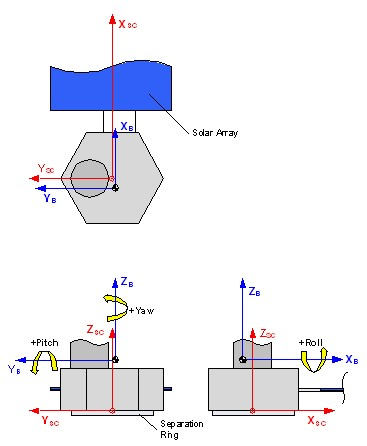
\includegraphics[width=6cm]{images/bodyframe.jpg} 
\caption{Orientation of the Body frame on the ACS.}
\label{bodyframe}
\end{center}
\end{figure} 

For the pointing jitter database we will be using the difference between the "Commanded pointing", $Q_C$, and the "Actual Pointing", $Q_A$. The difference quaternion, $Q_\Delta$, is given by
\begin{eqnarray}
Q_C^{-1}*Q_\Delta &=& Q_A^{-1} \\
Q_\Delta &=& Q_A^{-1}*Q_C \qquad ,
\end{eqnarray}
where the use of the inverses is to ensure that the quaternions, $Q_A$ and $Q_C$, are from Body to Inertial, and the delta quaternion, $Q_\Delta$, is a vector rotation in the Inertial frame. Figure \ref{deltaq} shows the magnitude of the pointing jitter in Ra and Dec for a Cassiopeia pointing at Ra = 350.8583$^\circ$ and Dec = 58.8175$^\circ$. It should be noted that the magnitude in Ra is large because of the high elevation.

\begin{figure}[th]
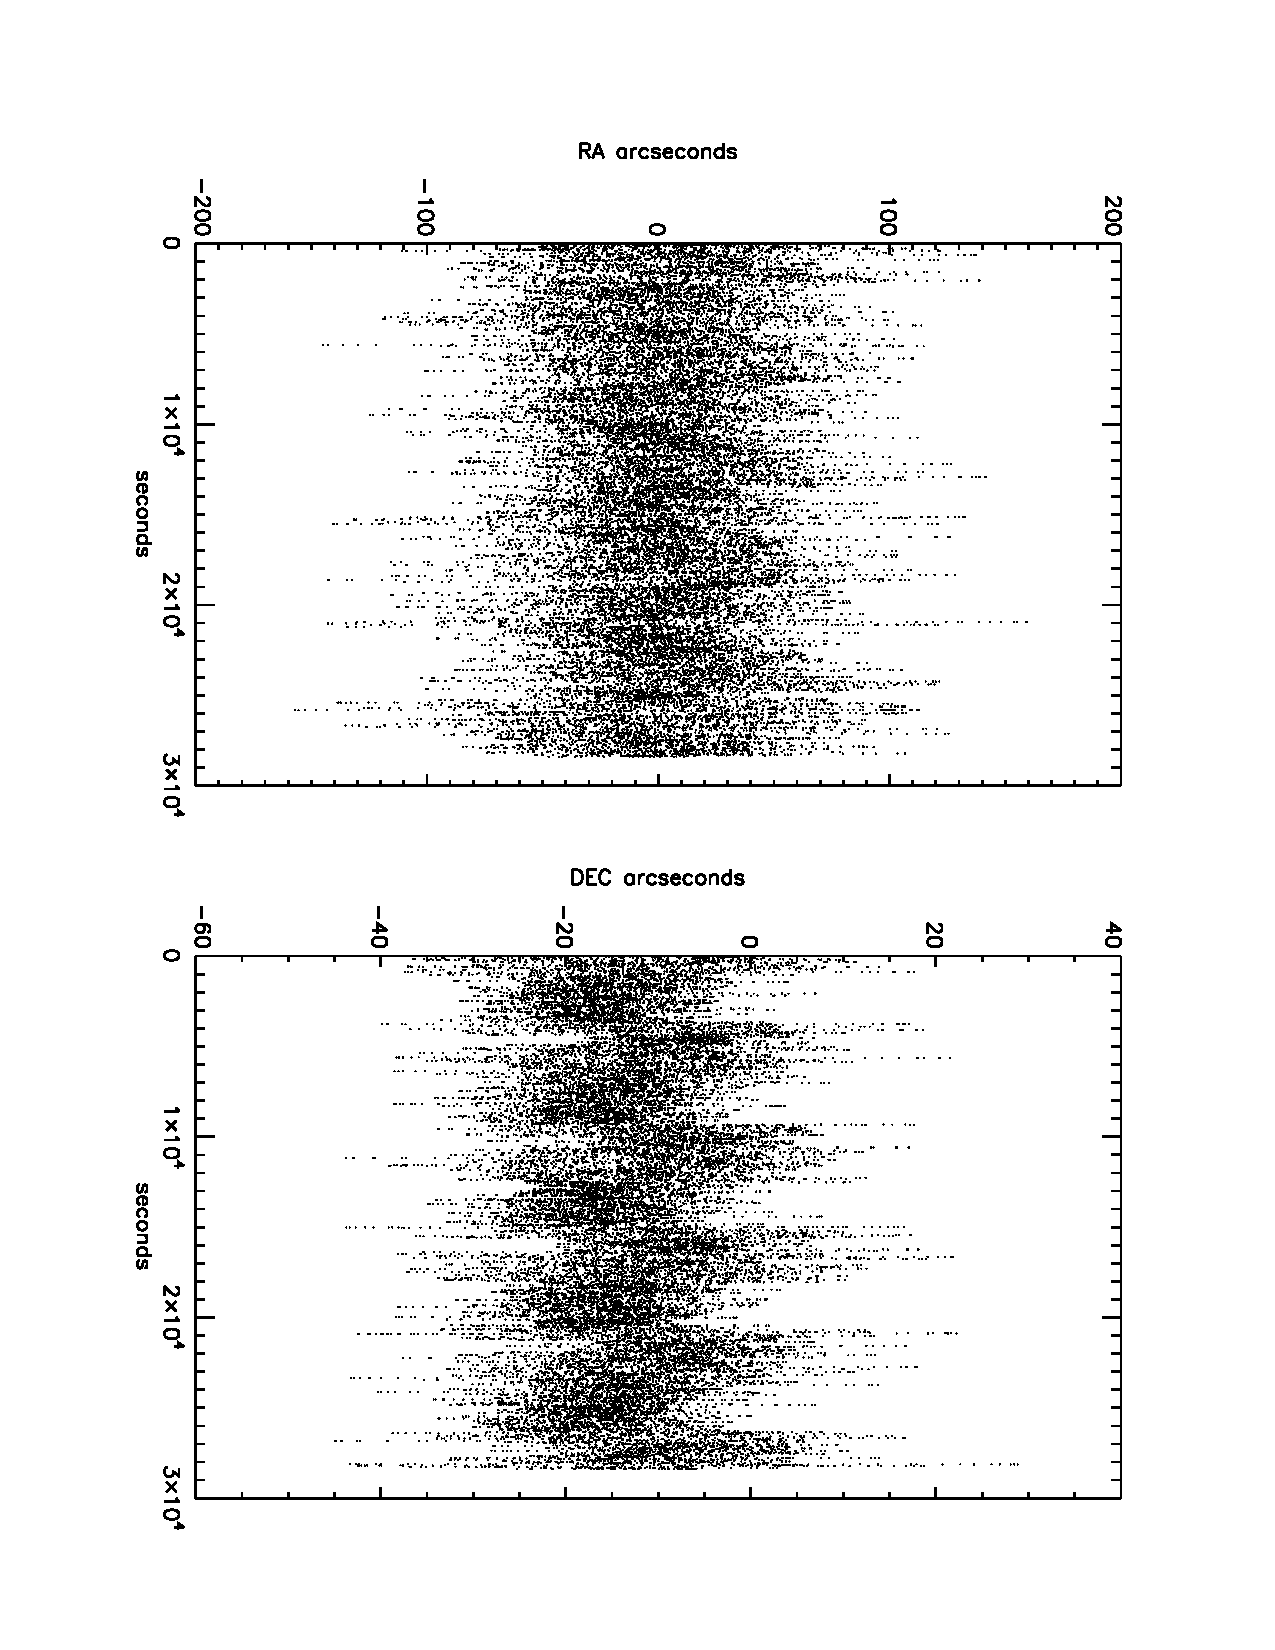
\includegraphics[width=10cm, angle=90]{images/Qdelta.pdf} 
\label{deltaq}
\caption{Delta quaternion between actual pointing and desired pointing expressed in delta Ra and Dec around a Cassiopeia pointing of Ra = 350.8583$^\circ$ and Dec = 58.8175$^\circ$.}
\end{figure}

\subsection{Implementation in NuSim}
The resulting delta quaternion, $Q_\Delta$, is in NuSim multiplied with the absolute pointing quaternion, $Q_P$. Because the quaternion is a vector rotation the resulting actual pointing is $Q_A = Q_P * Q_\Delta$. The source code can be found in NModulePointingPredefined.cxx

\subsection{Pointing Jitter DB format}
The delta quaternion, $Q_\Delta$, is stored in the same basic csv format as the perturbed data bases. the header is:
\begin{verbatim}
dt=,	1			
step,	q1,	q2,	q3,	q4
\end{verbatim}
where q1 - q3 is the vector part of the quaternion and q4 the real part. 

\subsection{Verification in NuSim}
Figure \ref{jitterfig} shows the NuSim output of a single pointing, using infinite detector resolution, perfect mirrors, and no mast deformation database. All error terms in the metrology and star tracker modules were also turned off. The two plots show the delta movement of the source across the detector in the detector X-axis direction and Y-axis direction for approximately two orbits. The orbital pattern can clearly be seen, and the magnitude of the movement is consistent with what was found for the input database.

\begin{figure}
\begin{tabular}{c}
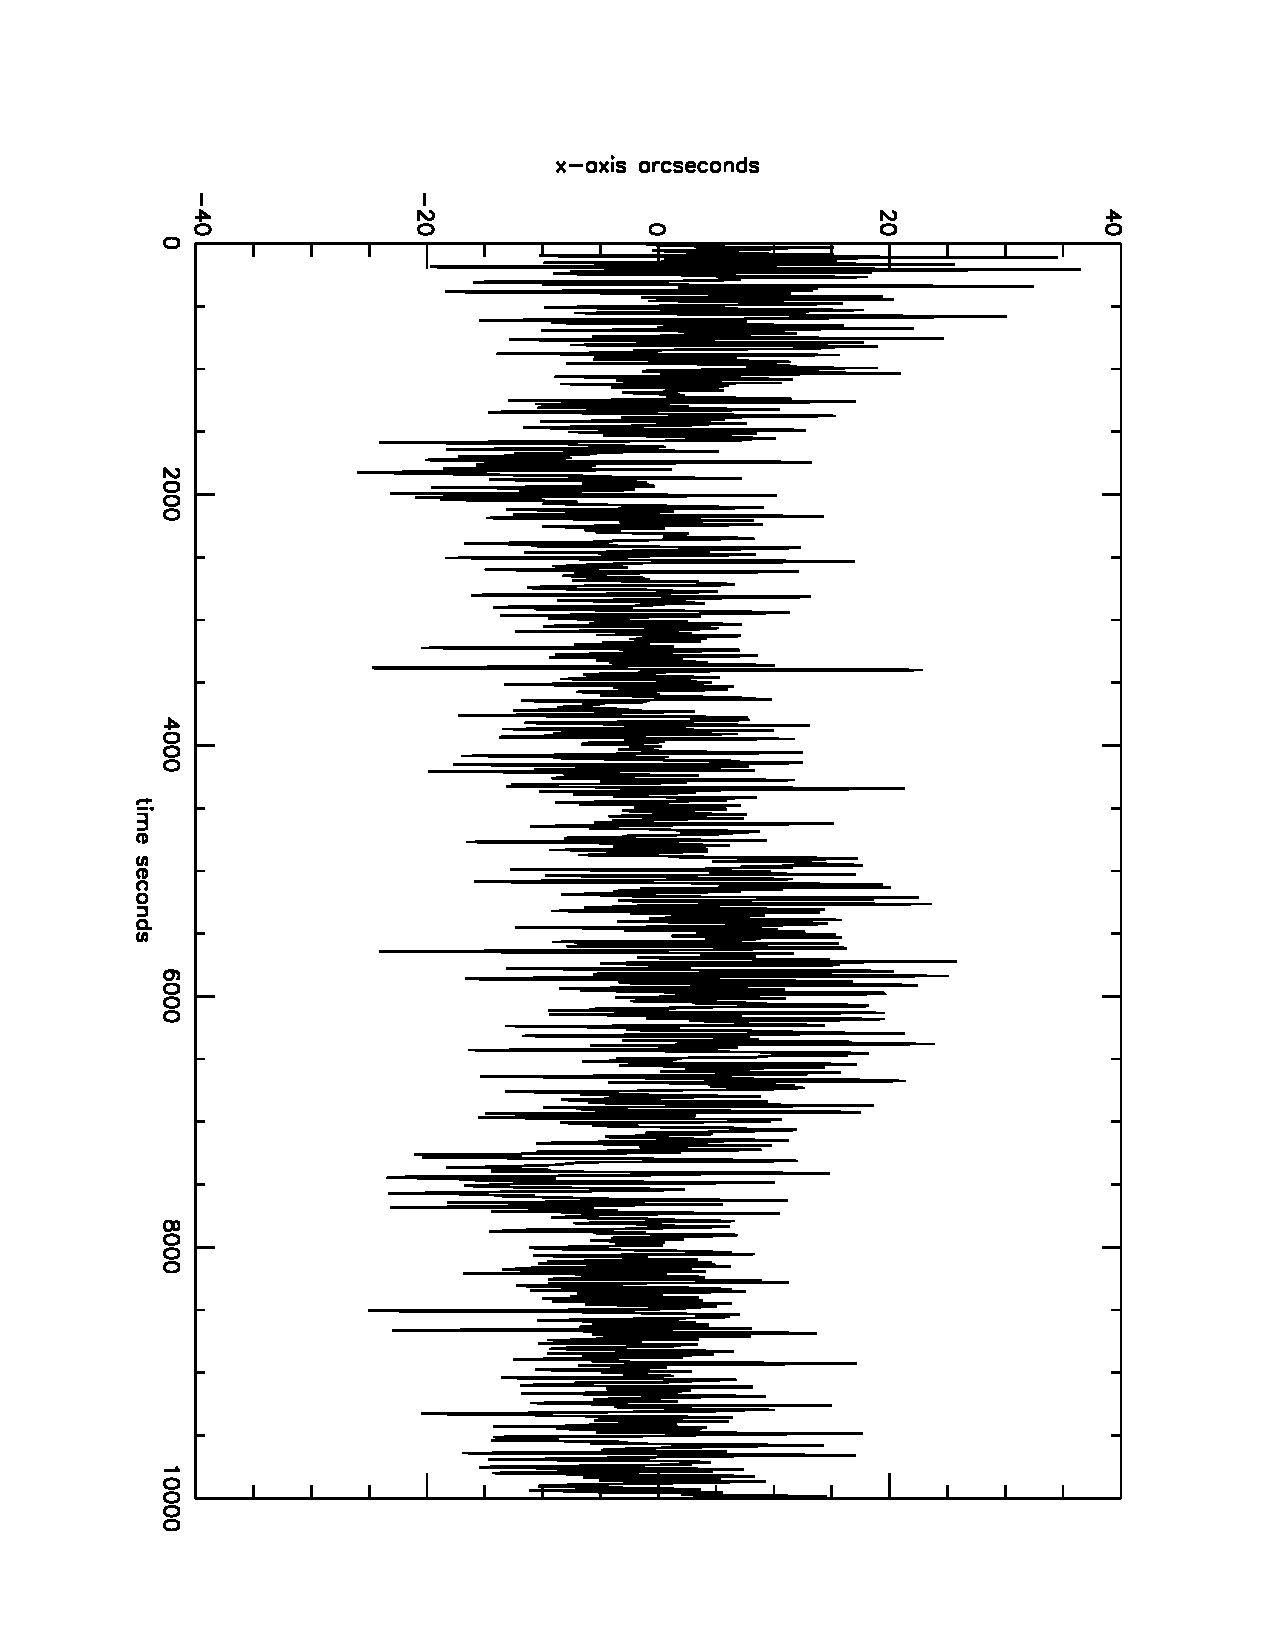
\includegraphics[width=10cm, angle=90]{images/jitter_x.pdf} \\
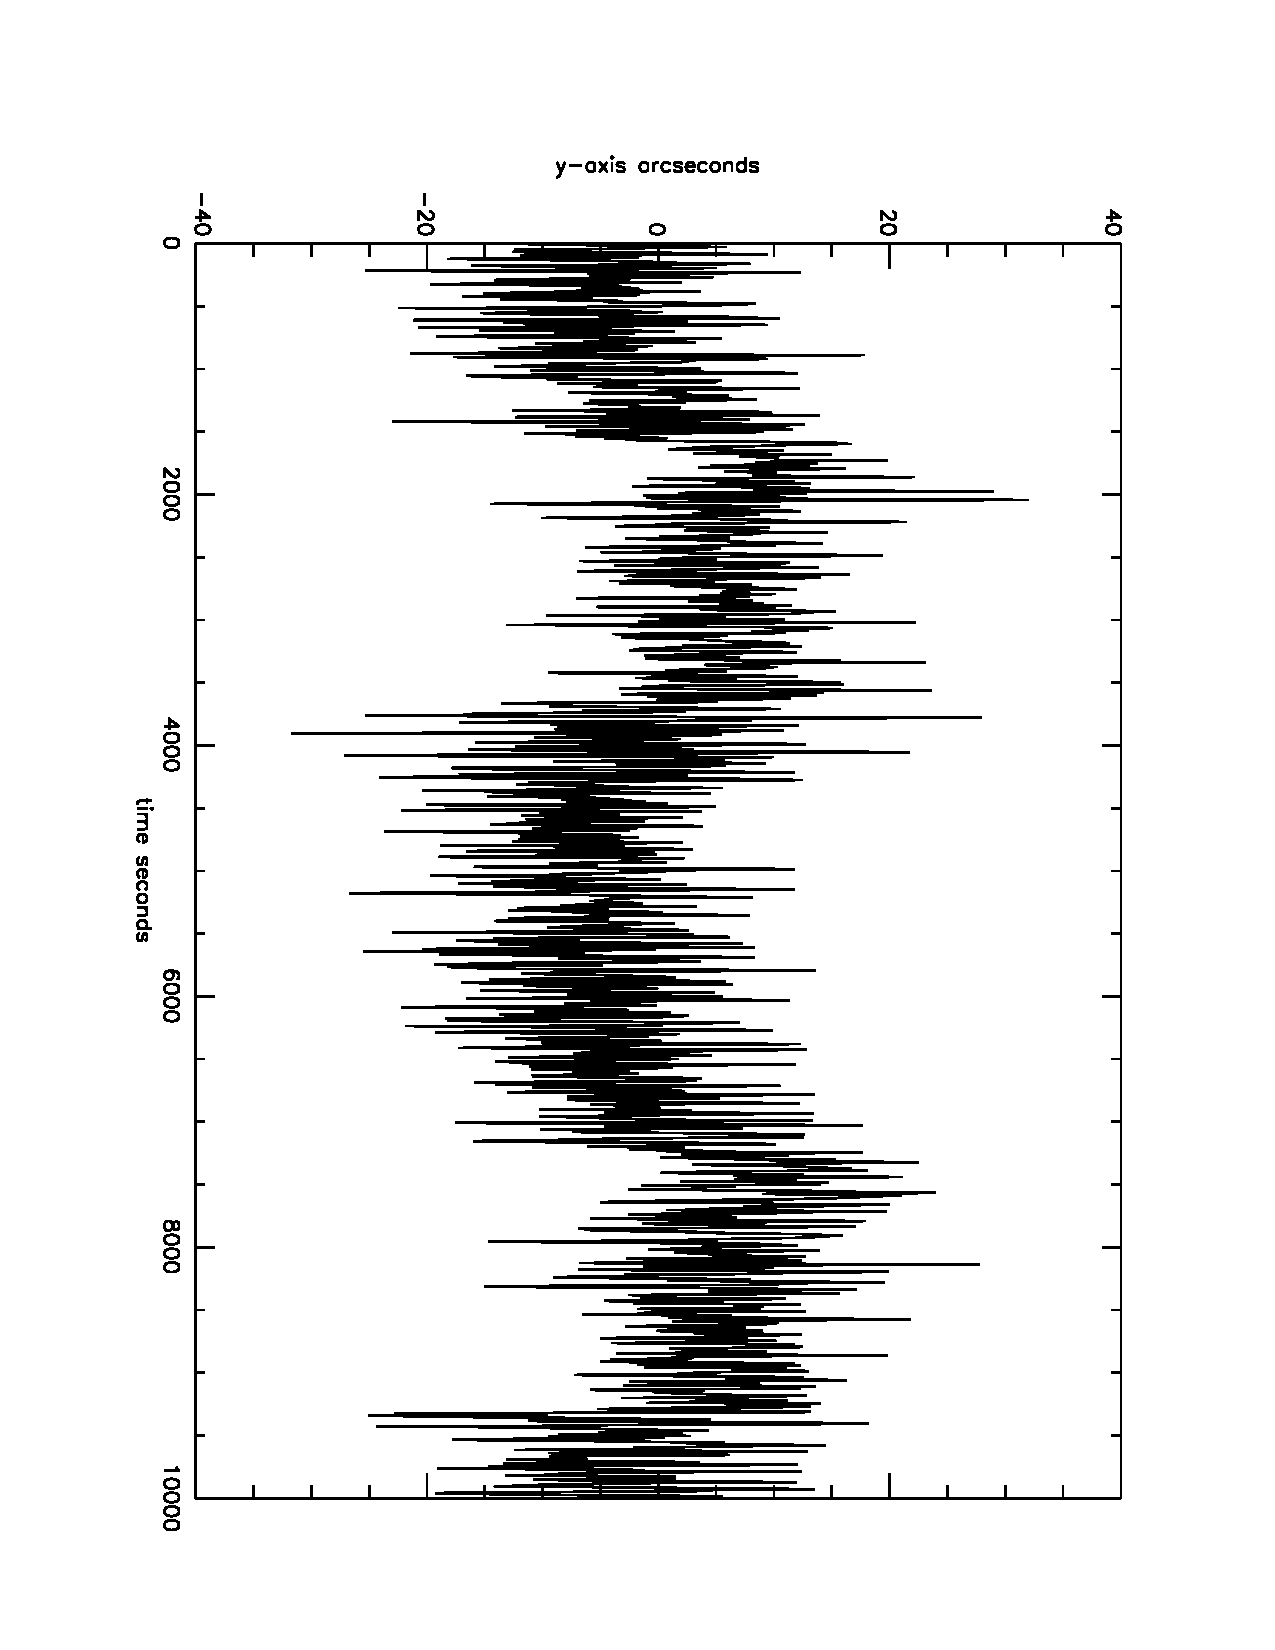
\includegraphics[width=10cm, angle=90]{images/jitter_y.pdf} 
\end{tabular}
\label{jitterfig}
\caption{Top: Movement of source in detector x coordinate. Bottom: Movement of source in y coordinate.}
\end{figure}

%\end{document}